\subsubsection{Radiales Menü}
{\color{red} TODO: Reihenfolge komisch - erst erzählen was radiales menü und marking menü ist oder erst erzählen warum man das gewählt hat und dann darauf eingehen, was das ist - wenn zuerst erklärung kommt, fällt man irgendwie mit der Tür ins Haus -> Entscheidung treffen}

Als zentrale Interaktionsschnittstelle wurde ein radiales Menü gewählt, da es im Vergleich zu linearen Menüs eine schnellere, weniger ermüdende und insgesamt angenehmere Nutzung ermöglicht \parencite{Mao2024comparisonOfPanelAndPieMenusForMidAirInteractionInPhotoBooth, callahan1988comparisonPieVsLinearMenus}. Radiale Menüs ordnen Funktionen kreisförmig um einen zentralen Punkt an. Wird die Auswahl über gerichtete Gestenbewegungen realisiert, werden sie als Marking Menus bezeichnet \parencite{kurtenbachbuxton1993markingmenus, kurtenbachPaul1993theDesignAndEvaluationOfMarkingMenus}.

Für Mid-Air-Interaktionen bieten radiale Menüs mehrere Vorteile. Die gleichmäßige Anordnung der Menüelemente führt zu kurzen und in alle Richtungen gleich langen Zielwegen, wodurch Auswahlbewegungen im dreidimensionalen Raum vergleichsweise einfach ausführbar sind. Zudem unterstützen sie sowohl eine visuelle als auch eine gestenbasierte Interaktion \parencite{kurtenbachbuxton1993markingmenus, kurtenbachPaul1993theDesignAndEvaluationOfMarkingMenus}.

Ein weiterer Vorteil liegt in der Möglichkeit, Auswahlbewegungen über räumliches Muskelgedächtnis zu erlernen. Mit zunehmender Nutzung können häufig verwendete Funktionen durch eingeübte Bewegungen ausgewählt werden, ohne dass eine visuelle Kontrolle erforderlich ist \parencite{kurtenbachbuxton1993markingmenus}.

{\color{red} TODO: Hier könnte auch abschnitt über Menüpositionierung rein - eher hier oder in Handtracking (?) - tendenz handtracking}

Die Anzahl der gleichzeitig sichtbaren Menüsegmente beeinflusst die Auswahlgeschwindigkeit sowie die Genauigkeit der Interaktion. Studien zu radialen Menüs zeigen, dass eine moderate Anzahl von Segmenten pro Ebene die effizienteste Bedienung ermöglicht \parencite{li2021depthandbreadthofpiemenusformidairgesdtureinteraction}.
Eine hohe Anzahl von Segmenten führt dazu, dass die einzelnen Einträge zunehmend kleiner werden. Dadurch verringert sich sowohl der verfügbare Platz für Beschriftungen als auch die Interaktionsfläche für den Cursor, was die präzise Auswahl erschwert. Dieses Problem ist vergleichbar mit dem sogenannten Fat-Finger-Effekt bei Touch-Interfaces, bei dem zu kleine Interaktionsflächen die Eingabegenauigkeit reduzieren.

Insbesondere bei Mid-Air-Interaktionen ist eine ausreichende Größe der Zielbereiche entscheidend, da Bewegungen mit dem Arm im Vergleich zu Maus- oder Touch-Eingaben eine geringere Präzision aufweisen \parencite{tao2024ergonomicAssessmentOfMidAirInteractionAndDeviceAssistedInteractionsUnderVibrationEnvironments}.

{\color{red} TODO: das eher in teil praktische umsetzung?}
Da die Menüstruktur durch die jeweilige Zielanwendung
definiert wird, beschränkt das Interaktionssystem die Anzahl
der Menüsegmente nicht strikt. Stattdessen wird bei einer
größeren Menütiefe ein Hinweis ausgegeben, der auf mögliche
Usability-Probleme hinweist.
Dieses Vorgehen ermöglicht einerseits eine flexible Anpassung
der Menüstruktur durch die Zielanwendung, während gleichzeitig
Gestaltungsrichtlinien für eine ergonomische Nutzung des
radialen Menüs berücksichtigt werden.


\subsubsection{Auswahlmechanismen} 
Für die Auswahl von Menüeinträgen wurden zwei unterschiedliche Interaktionsmechanismen vorgesehen: eine aktive Greifgeste sowie eine zeitbasierte Auswahl (Dwell Selection).

Bei der Dwell-basierten Auswahl wird ein Menüeintrag automatisch aktiviert, wenn der Cursor für eine definierte Zeitspanne über dem Element verweilt. Dieser Mechanismus reduziert die motorischen Anforderungen an präzise Gesten und ermöglicht eine niedrigschwellige Interaktion insbesondere für unerfahrene Nutzer:innen. Studien zeigen auch, dass Dwell-Auswahlmethoden keine Einführung brauchen sondern vom Nutzer selbst erkannt werden können \parencite{walterBaillyValkanova2014CuenesicsUsingMidAirGesturesToSelectItemsOnInteractivePublicDisplays}.

Zusätzlich wurde eine Greifgeste als explizite Auswahlmethode vorgesehen. Solche pantomimischen Gesten, die physische Handlungen wie das Greifen nachahmen, gelten als besonders intuitiv und leicht erlernbar \parencite{kostic2024exploringmidairhandinteractionindatavisualization}. Um die Erlernbarkeit zu unterstützen, wird die Geste durch einen visuellen Hinweis (Abb. \ref{fig:grab_hint}) eingeführt, was die Guessability (Erratbarkeit) der Interaktion erhöht \parencite{wobbrock2005discoverability}.

\begin{figure}[H]
    \centering
    
\includegraphics[width=0.5\linewidth]{content/images/grab_hint.png}
    \caption{Hinweisanimation, die Nutzer:innen zeigt, wie Dwell-Zeit übersprungen werden kann. {\color{red} TODO: Visualisierung eher in Abschnitt visuelle Gestaltung?}}
    \label{fig:grab_hint}
\end{figure}

Durch die Kombination beider Mechanismen kann das System sowohl für Einsteiger als auch für erfahrene Nutzer:innen unterschiedliche Interaktionsstile unterstützen.


\subsubsection{Visuelle Gestaltung und Zustandsrückmeldungen}


{\color{red} TODO: Grab hint eher in diesen abschnitt? ODer vielleiht den abschnitt direkt mit in auswahlmechanismen abschnitt?}

{\color{red} TODO:erwähnen: styling ist iterativer Prozess, aber kein Fokus}

 ÜBERGANG/EINTLEITUNG
Es wurden mehrere visuelle Zustände implementiert, um den aktuellen Interaktionsstatus nachvollziehbar darzustellen. Befindet sich der Cursor über einem Menüsegment, wird dieses visuell hervorgehoben (Hover-Zustand, vgl. Abb. \ref{fig:menu_state_hover}). Diese Hervorhebung dient als unmittelbare Rückmeldung darüber, welches Menüelement aktuell fokussiert ist.

Wird ein Menüeintrag aktiv ausgewählt, durch eine Greifgeste oder durch das Auslösen eines Dwell-Timers, wechselt das entsprechende Segment in einen ausgewählten Zustand (Abb. \ref{fig:menu_state_selected}), der durch eine deutlichere Farbänderung dargestellt wird.

Während der Dwell-basierten Auswahl wird zusätzlich eine visuelle Fortschrittsanzeige eingeblendet. 
Diese zeigt den zeitlichen Fortschritt der Aktivierung und ermöglicht es Nutzer:innen, den aktuellen Interaktionsstatus besser einzuschätzen (Abb. \ref{fig:menu_state_dwell}).

\begin{figure}[htbp]
\centering
\begin{subfigure}{0.32\textwidth}
    \centering
    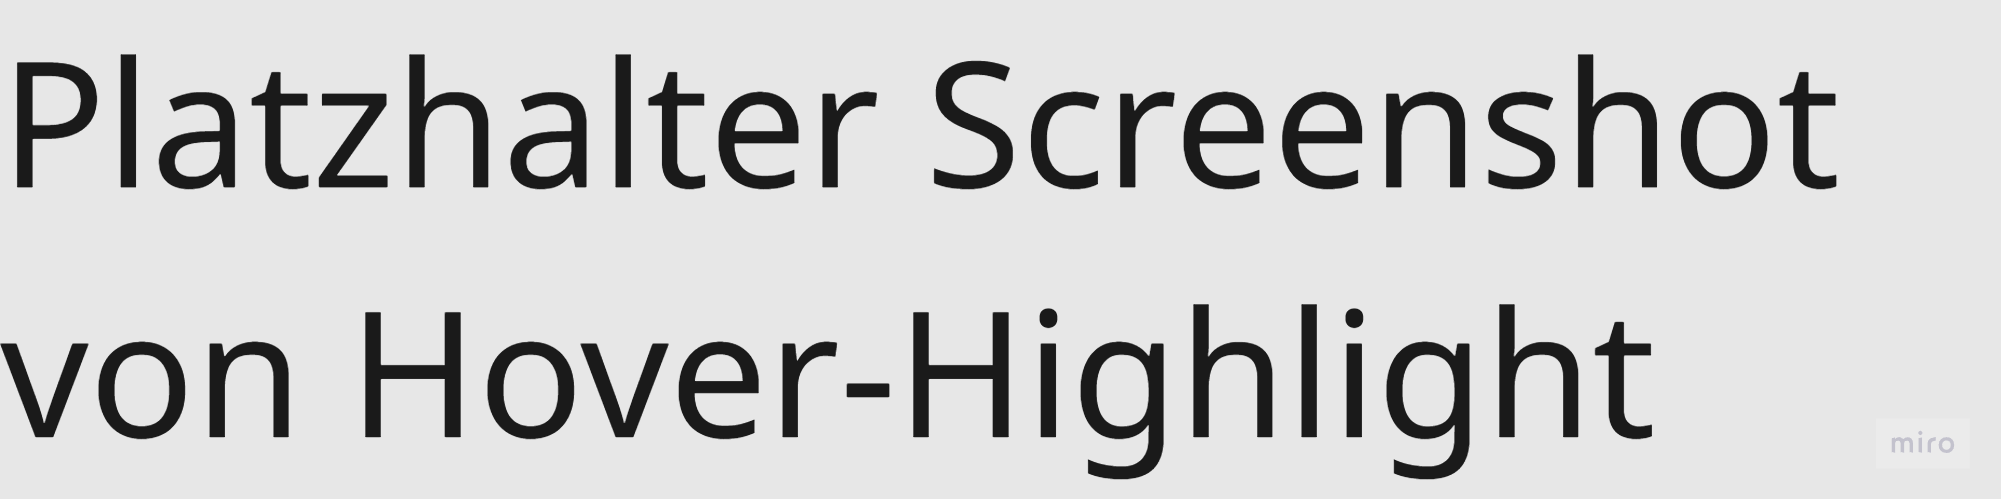
\includegraphics[width=\linewidth]{content/images/menu_state_hover.png}
    \caption{Hover-Zustand}
    \label{fig:menu_state_hover}
\end{subfigure}
\hfill
\begin{subfigure}{0.32\textwidth}
    \centering
    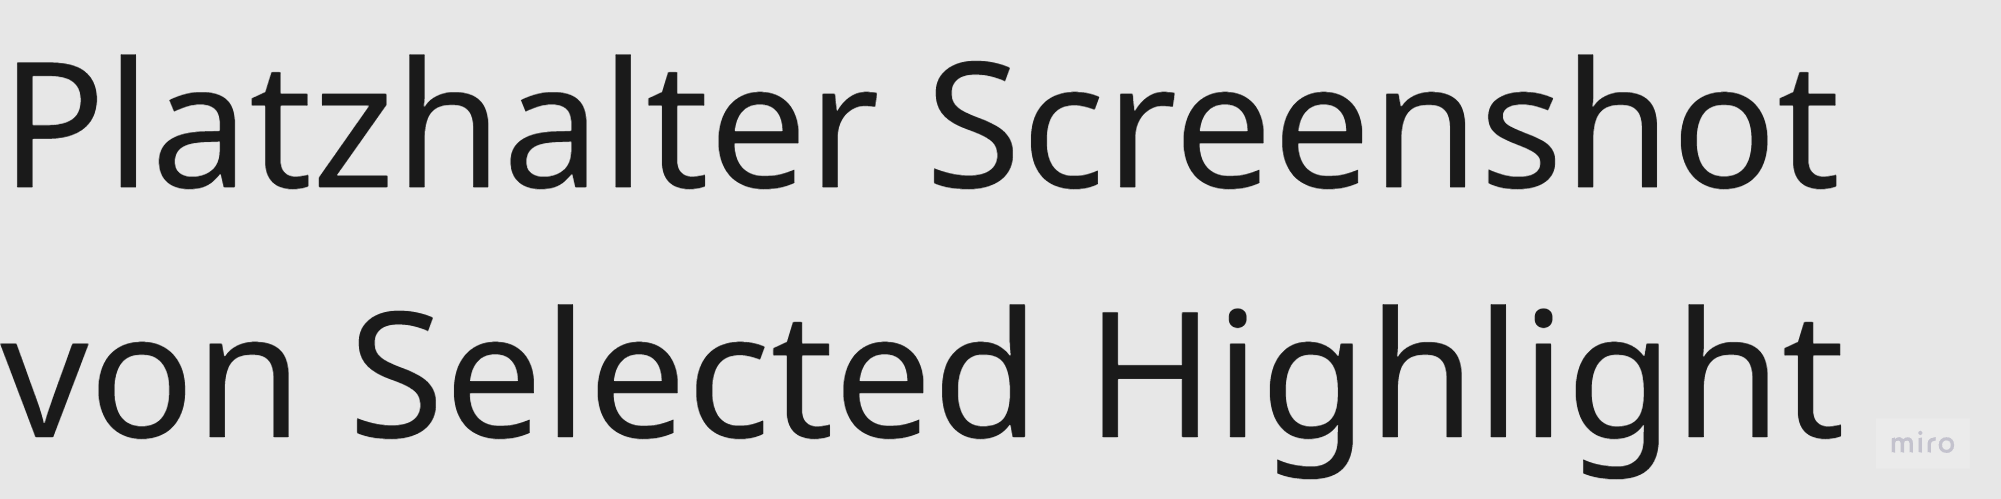
\includegraphics[width=\linewidth]{content/images/menu_state_selected.png}
    \caption{Selected-Zustand}
    \label{fig:menu_state_selected}
\end{subfigure}
\hfill
\begin{subfigure}{0.32\textwidth}
    \centering
    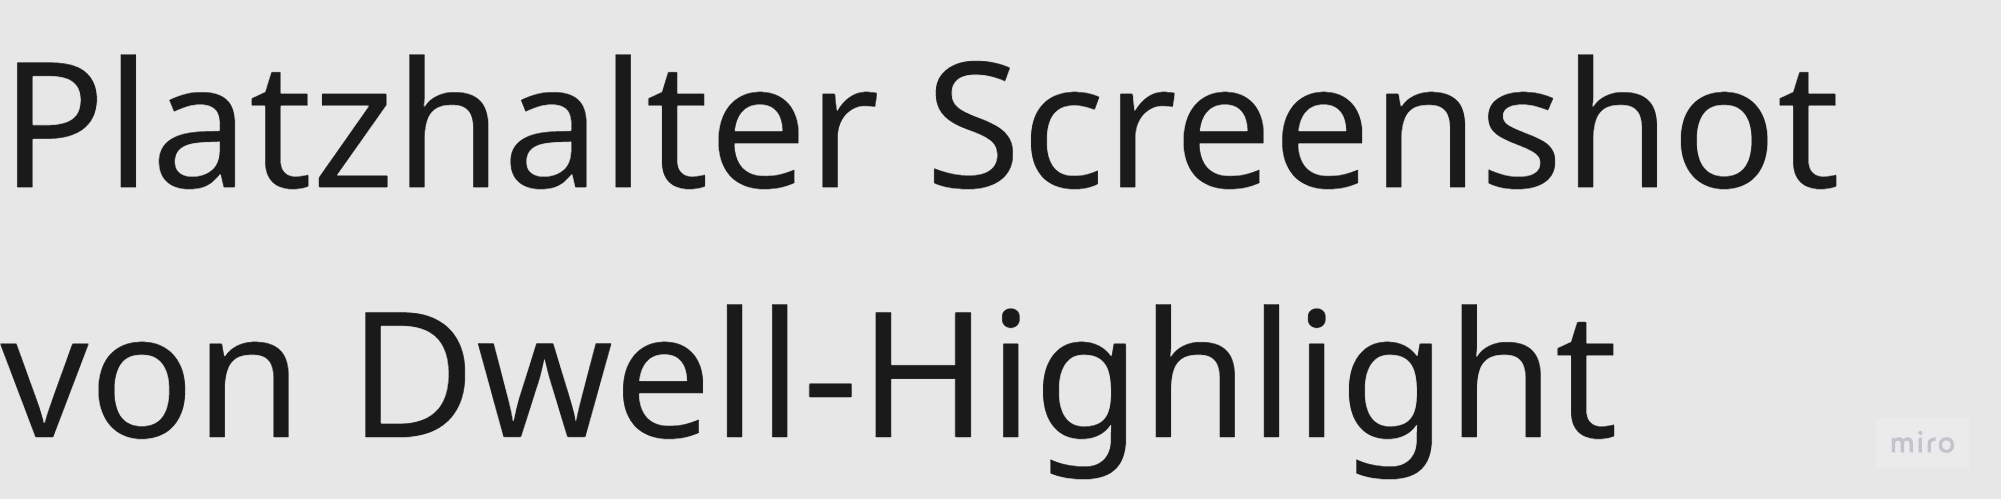
\includegraphics[width=\linewidth]{content/images/menu_state_dwell.png}
    \caption{Dwell-Animation}
    \label{fig:menu_state_dwell}
\end{subfigure}
\caption{Darstellungen der verschiedenen Menü-Item-Zustände}
\label{fig:menu_states}
\end{figure}


\subsubsection{Submenus}
Um eine größere Anzahl von Funktionen innerhalb des Interaktionssystems zugänglich zu machen, wurde das radiale Menü um Submenüs erweitert. Einzelne Segmente des Hauptmenüs können weitere Menüebenen enthalten, die bei Auswahl eines Elements geöffnet werden.
Diese hierarchische Struktur ermöglicht es, thematisch zusammengehörige Funktionen zu gruppieren und gleichzeitig die visuelle Komplexität des Hauptmenüs zu reduzieren. 
Menüeinträge erfüllen dabei zwei unterschiedliche Rollen: Sie können entweder als Kategorie fungieren (Abb. \ref{fig:menu_item_opening_submenu}) und ein weiteres Untermenü öffnen oder direkt eine Interaktion auslösen. Solche Interaktionen können beispielsweise diskrete Aktionen (z. B. Button-Funktionen, vgl. Abb. \ref{fig:menu_item_being_button}) oder kontinuierliche Parametersteuerungen wie Slider umfassen (Abb. \ref{fig:menu_item_opening_slider}).
Durch diese mehrstufige Organisation bleibt die Anzahl der gleichzeitig sichtbaren Menüelemente begrenzt, wodurch die Orientierung im Menü erleichtert wird und die Interaktion auch im Mid-Air-Kontext übersichtlich bleibt. Gleichzeitig erlaubt die hierarchische Struktur eine flexible Erweiterung des Systems um zusätzliche Funktionen.

Obwohl \textcite{li2021depthandbreadthofpiemenusformidairgesdtureinteraction} optimale Werte für Breite und Tiefe von Menühierarchien zur Maximierung von Effizienz und Geschwindigkeit vorschlagen, werden diese im vorliegenden Kontext nicht strikt übernommen. Im MIR steht nicht die möglichst schnelle Ausführung von Aufgaben im Vordergrund, sondern eine intuitive, verständliche und in den Raum eingebettete Interaktion.

\begin{figure}[htbp]
\centering
\begin{subfigure}{0.32\textwidth}
    \centering
    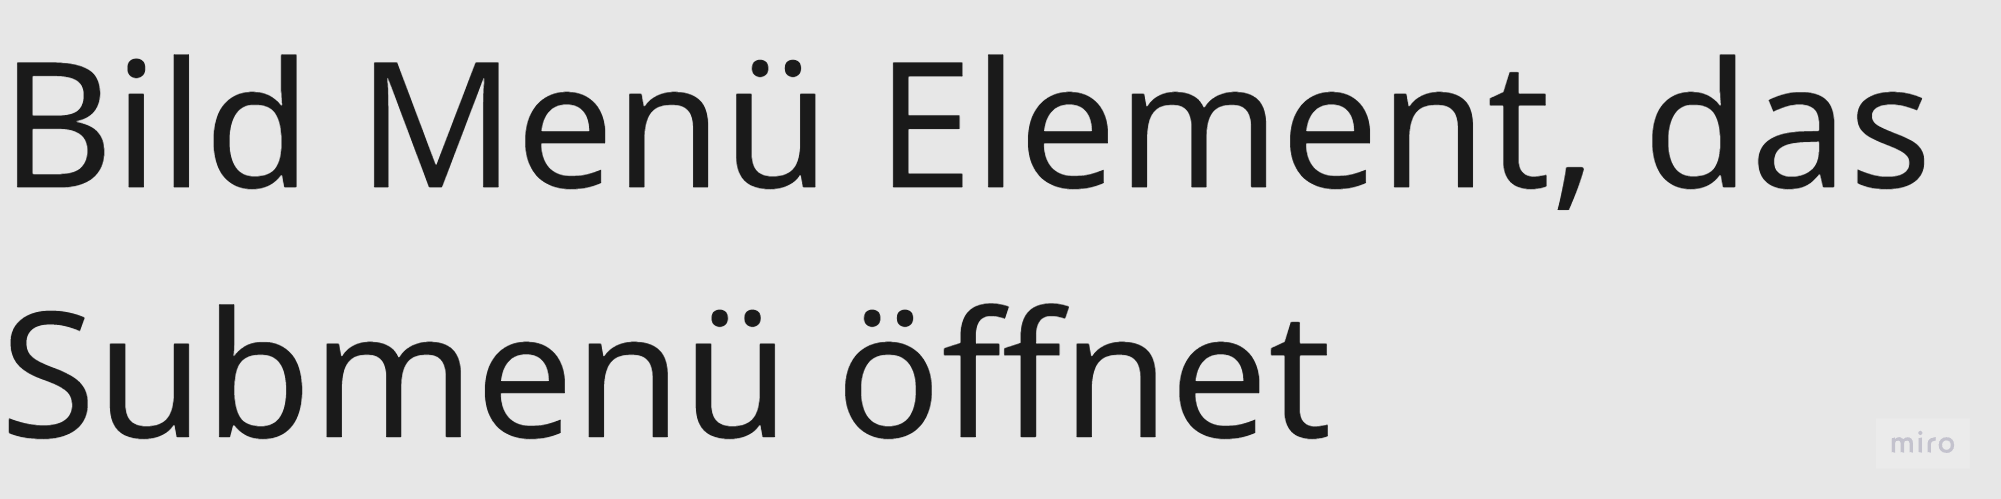
\includegraphics[width=\linewidth]{content/images/menu_item_opening_submenu.png}
    \caption{Menüeintrag, der Submenü öffnet}
    \label{fig:menu_item_opening_submenu}
\end{subfigure}
\hfill
\begin{subfigure}{0.32\textwidth}
    \centering
    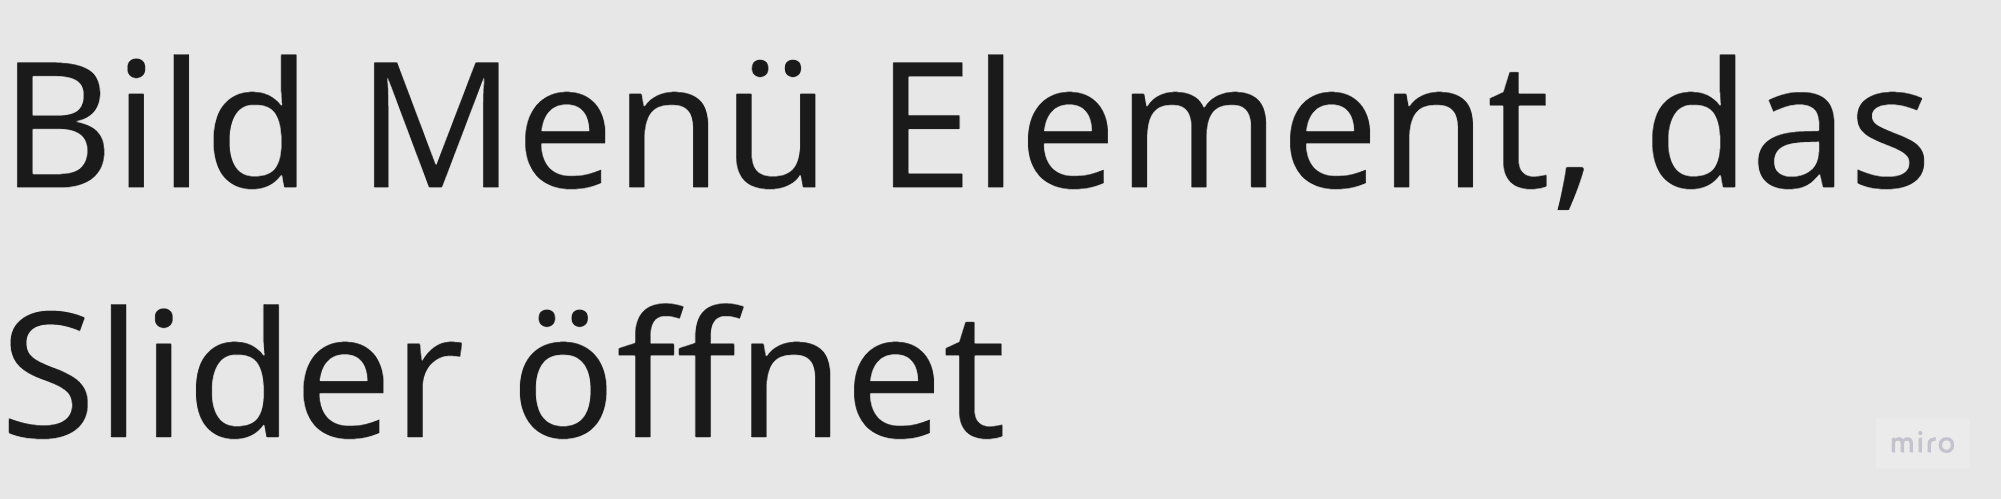
\includegraphics[width=\linewidth]{content/images/menu_item_opening_slider.png}
    \caption{Menüeintrag, der Slider öffnet}
    \label{fig:menu_item_opening_slider}
\end{subfigure}
\hfill
\begin{subfigure}{0.32\textwidth}
    \centering
    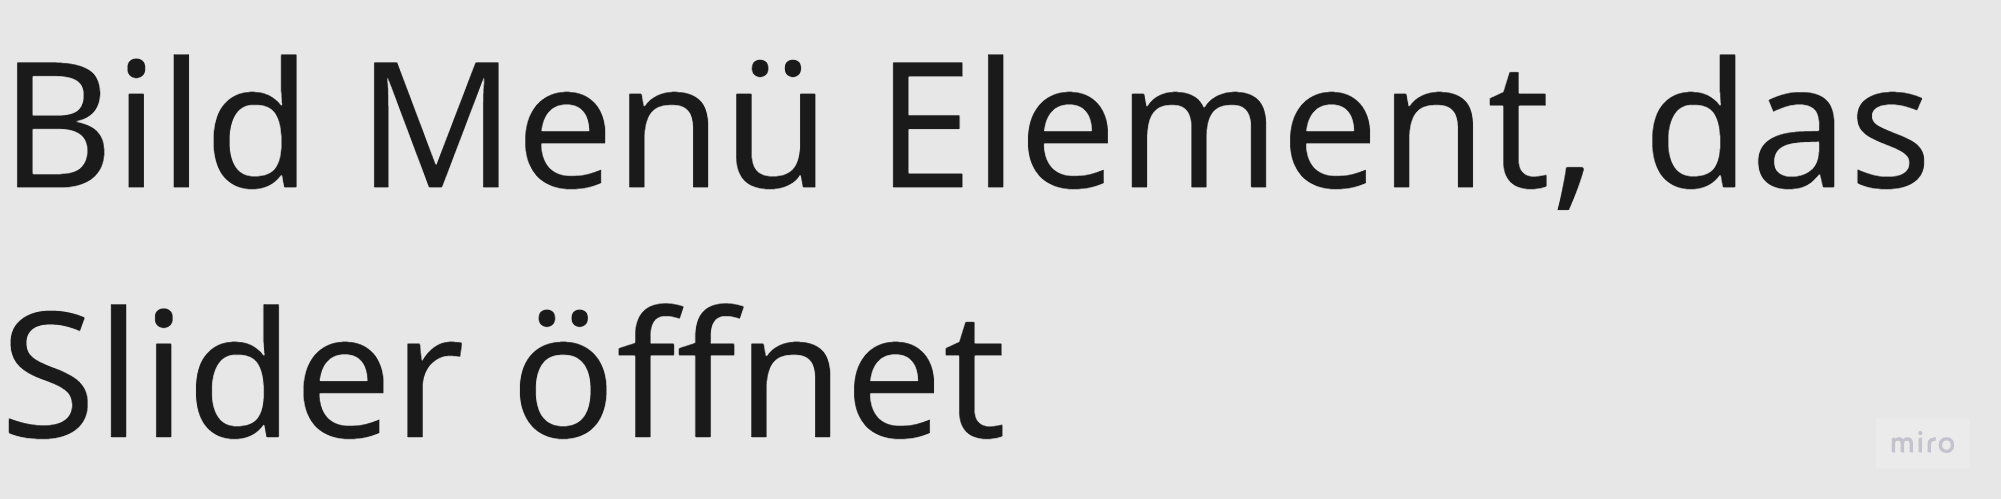
\includegraphics[width=\linewidth]{content/images/menu_item_opening_slider.png}
    \caption{Menüeintrag, der als Button fungiert}
    \label{fig:menu_item_being_button}
\end{subfigure}
\caption{Darstellungen der Menü-Item-Optionen}
\label{fig:menu_item_options}
\end{figure}

{\color{red} Ist das zu genau beschrieben? Ist das überhaupt interessant? Falls ja, braucht man dafür zusätzliche Visualisierung oder versteht man das?}
Zum Aktivieren eines Untermenüs selektieren die Nutzer:innen einen Menüeintrag, der in der Menüstruktur über Kindelemente verfügt. Solange sich der Cursor innerhalb dieses Eintrags oder des geöffneten Untermenüs befindet, bleibt das Untermenü sichtbar und kann weiter genutzt werden. 
Verlässt der Cursor sowohl den Menüeintrag als auch das zugehörige Untermenü, wird das Untermenü automatisch geschlossen. Durch diese kontextabhängige Sichtbarkeit bleibt die visuelle Komplexität des Menüs gering, während gleichzeitig eine größere Anzahl von Funktionen selektiv zugänglich gemacht werden kann.

\subsubsection{Slider}
% TODO Präsentationssteuerung erklären, bzw. aktuelle Targets zeigen? 
Menüeinträge können entweder diskrete Aktionen auslösen oder eine kontinuierliche Parametersteuerung ermöglichen. Diskrete Aktionen werden als Buttons dargestellt, während kontinuierliche Parameter über Slider angepasst werden können.

Typische Anwendungsfälle für Slider sind beispielsweise die Steuerung von Lautstärke, Helligkeit oder Intensität von Effekten. Beim Auswählen eines entsprechenden Menüelements wird zunächst eine visuelle Vorschau des Reglers angezeigt (Abb.~\ref{fig:slider_preview}), die einen Hinweis auf die folgende Interaktionsmöglichkeit gibt (QUELLE?). Die reduzierte visuelle Hervorhebung signalisiert dabei, dass zunächst eine explizite Auswahl erforderlich ist, um den Slider zu aktivieren. Nach Bestätigung der Auswahl wechselt das System in einen Anpassungsmodus, in dem der Parameter direkt verändert werden kann (Abb.~\ref{fig:slider_active}). In diesem Modus wird das Menü visuell zurückgenommen und der Cursor ausgeblendet, um den Fokus auf die Sliderinteraktion zu lenken.

Die Steuerung erfolgt über eine gezielte Handbewegung entlang einer definierten Interaktionsachse. Diese wird durch eine Pinch-Geste aktiviert, bei der Nutzer:innen den Parameter durch Verschieben der Hand entlang der jeweiligen Achse verändern. Um die Discoverability der Interaktion zu verbessern, wird im Sliderbereich eine visuelle Anleitung eingeblendet, die die Pinch-Geste sowie die mögliche Bewegungsrichtung durch Pfeile verdeutlicht. Diese visuelle Unterstützung reduziert die kognitive Belastung und erleichtert insbesondere Erstnutzer:innen den Einstieg in die Interaktion.

Die Kombination aus einer einfachen Aktivierungsgeste und einer anschließenden gerichteten Bewegung entspricht etablierten Interaktionsprinzipien, bei denen sogenannte Microgestures mit kurzen Richtungsbewegungen (Marks) kombiniert werden. Solche Ansätze zeichnen sich durch eine geringe physische Belastung, eine hohe Erlernbarkeit sowie eine reduzierte visuelle Komplexität aus und eignen sich daher besonders für Mid-Air-Interaktionen \parencite{baillyPometti2024MarkARExploringTheBenefitsOfCombiningMicrogesturesAndMidAirMarksToTriggerCommandsInAR}.

Gleichzeitig greift die Interaktion eine vertraute physische Metapher auf: Das Verschieben des Sliders entspricht dem Greifen und Bewegen eines realen Reglers. Diese räumliche Analogie unterstützt eine intuitive Bedienung und ermöglicht es Nutzer:innen, die Interaktion durch Lösen der Pinch-Geste jederzeit zu beenden, wodurch eine kontrollierte und leicht verständliche Anpassung der Werte entsteht.

Je nach Kontext und Menüeintrag wird die Position des Sliders relativ zum Menü angepasst. Der Slider kann dabei oberhalb, unterhalb oder seitlich des Menüs erscheinen, wodurch sich entweder eine horizontale oder vertikale Interaktionsachse ergibt. Entsprechend wird die Pinch-Geste entlang dieser Achse ausgeführt, sodass eine konsistente räumliche Zuordnung zwischen visueller Darstellung und Interaktionsbewegung entsteht.

Durch die Integration solcher Slider lassen sich kontinuierliche Parameter innerhalb des Interaktionssystems einheitlich steuern.

{\color{red} TODO:brauche ich allgemeinen Abschnitt wo ich anforderungen an gute Gesten erkläre?zB wie was bailly2024 nutzt: Quick and subtle, comforrtable, focused on meeting content, easy to learn for novices}

\begin{figure}[htbp]
\centering
\begin{subfigure}{0.49\textwidth}
    \centering
    
\includegraphics[width=\linewidth]{content/images/slider_preview.png}
    \caption{Vorschau}
    \label{fig:slider_preview}
\end{subfigure}
\hfill
\begin{subfigure}{0.49\textwidth}
    \centering
    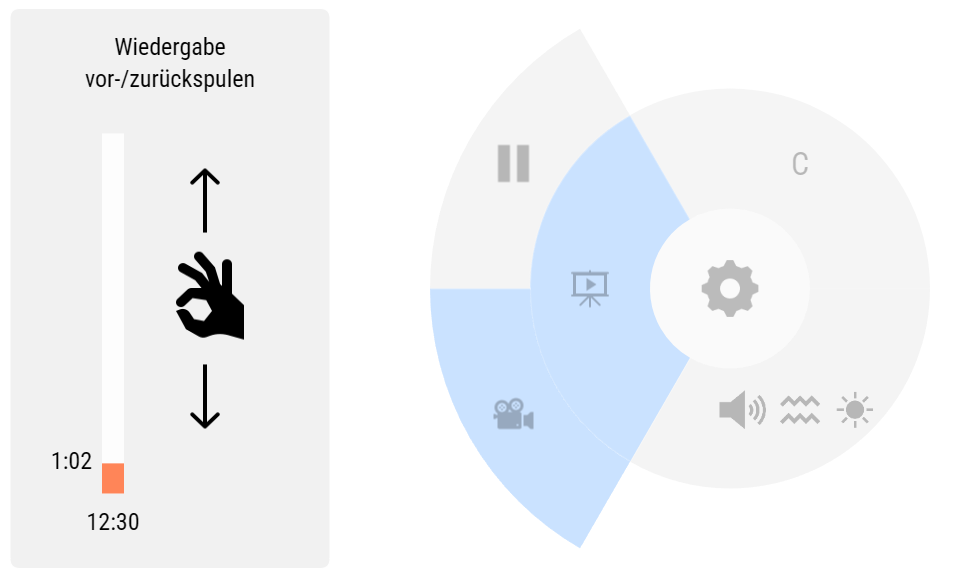
\includegraphics[width=\linewidth]{content/images/slider_active.png}
    \caption{Aktiver Zustand}
    \label{fig:slider_active}
\end{subfigure}
\caption{Darstellungen der verschiedenen Slider-Zustände}
\label{fig:slider_states}
\end{figure}


\subsubsection{Beispiele aktueller Interaktionen}
{\color{red} TODO: überlegen ob button doch in extra abschnitt muss, aber denke eigentlich nicht, weil es gibt ja nur den einen => dann eher generalisierbarkeit als todo in den ausblick }


Die aktuell implementierten Interaktionen umfassen sowohl kontinuierliche Parametersteuerungen als auch diskrete Steuerungsfunktionen.

Ein zentraler Anwendungsfall für kontinuierliche Interaktion sind Slider zur Anpassung von Parametern wie Helligkeit, Vibration und Lautstärke. Diese werden in Form prozentualer Werte dargestellt und ermöglichen eine direkte, kontinuierliche Kontrolle der jeweiligen Systemparameter.


Darüber hinaus wird das Interaktionssystem zur Steuerung vorgerenderter Medieninhalte eingesetzt. In diesem Kontext dient ein Slider zur Navigation innerhalb eines Videos, indem er die aktuelle Abspielposition repräsentiert und gleichzeitig die Gesamtlänge des Materials visualisiert. Während der Wiedergabe bewegt sich der Slider automatisch entlang der Zeitleiste, wodurch der aktuelle Fortschritt kontinuierlich angezeigt wird.

Abbildung~\ref{fig:Slidertypen} zeigt beide Varianten im Vergleich. Während parameterbasierte Slider den aktuellen Wert als prozentuale Angabe darstellen, repräsentieren medienbezogene Slider eine zeitliche Position innerhalb eines Videos. Die zugrunde liegende Interaktionslogik bleibt dabei identisch.

\begin{figure}[H]
    \centering
    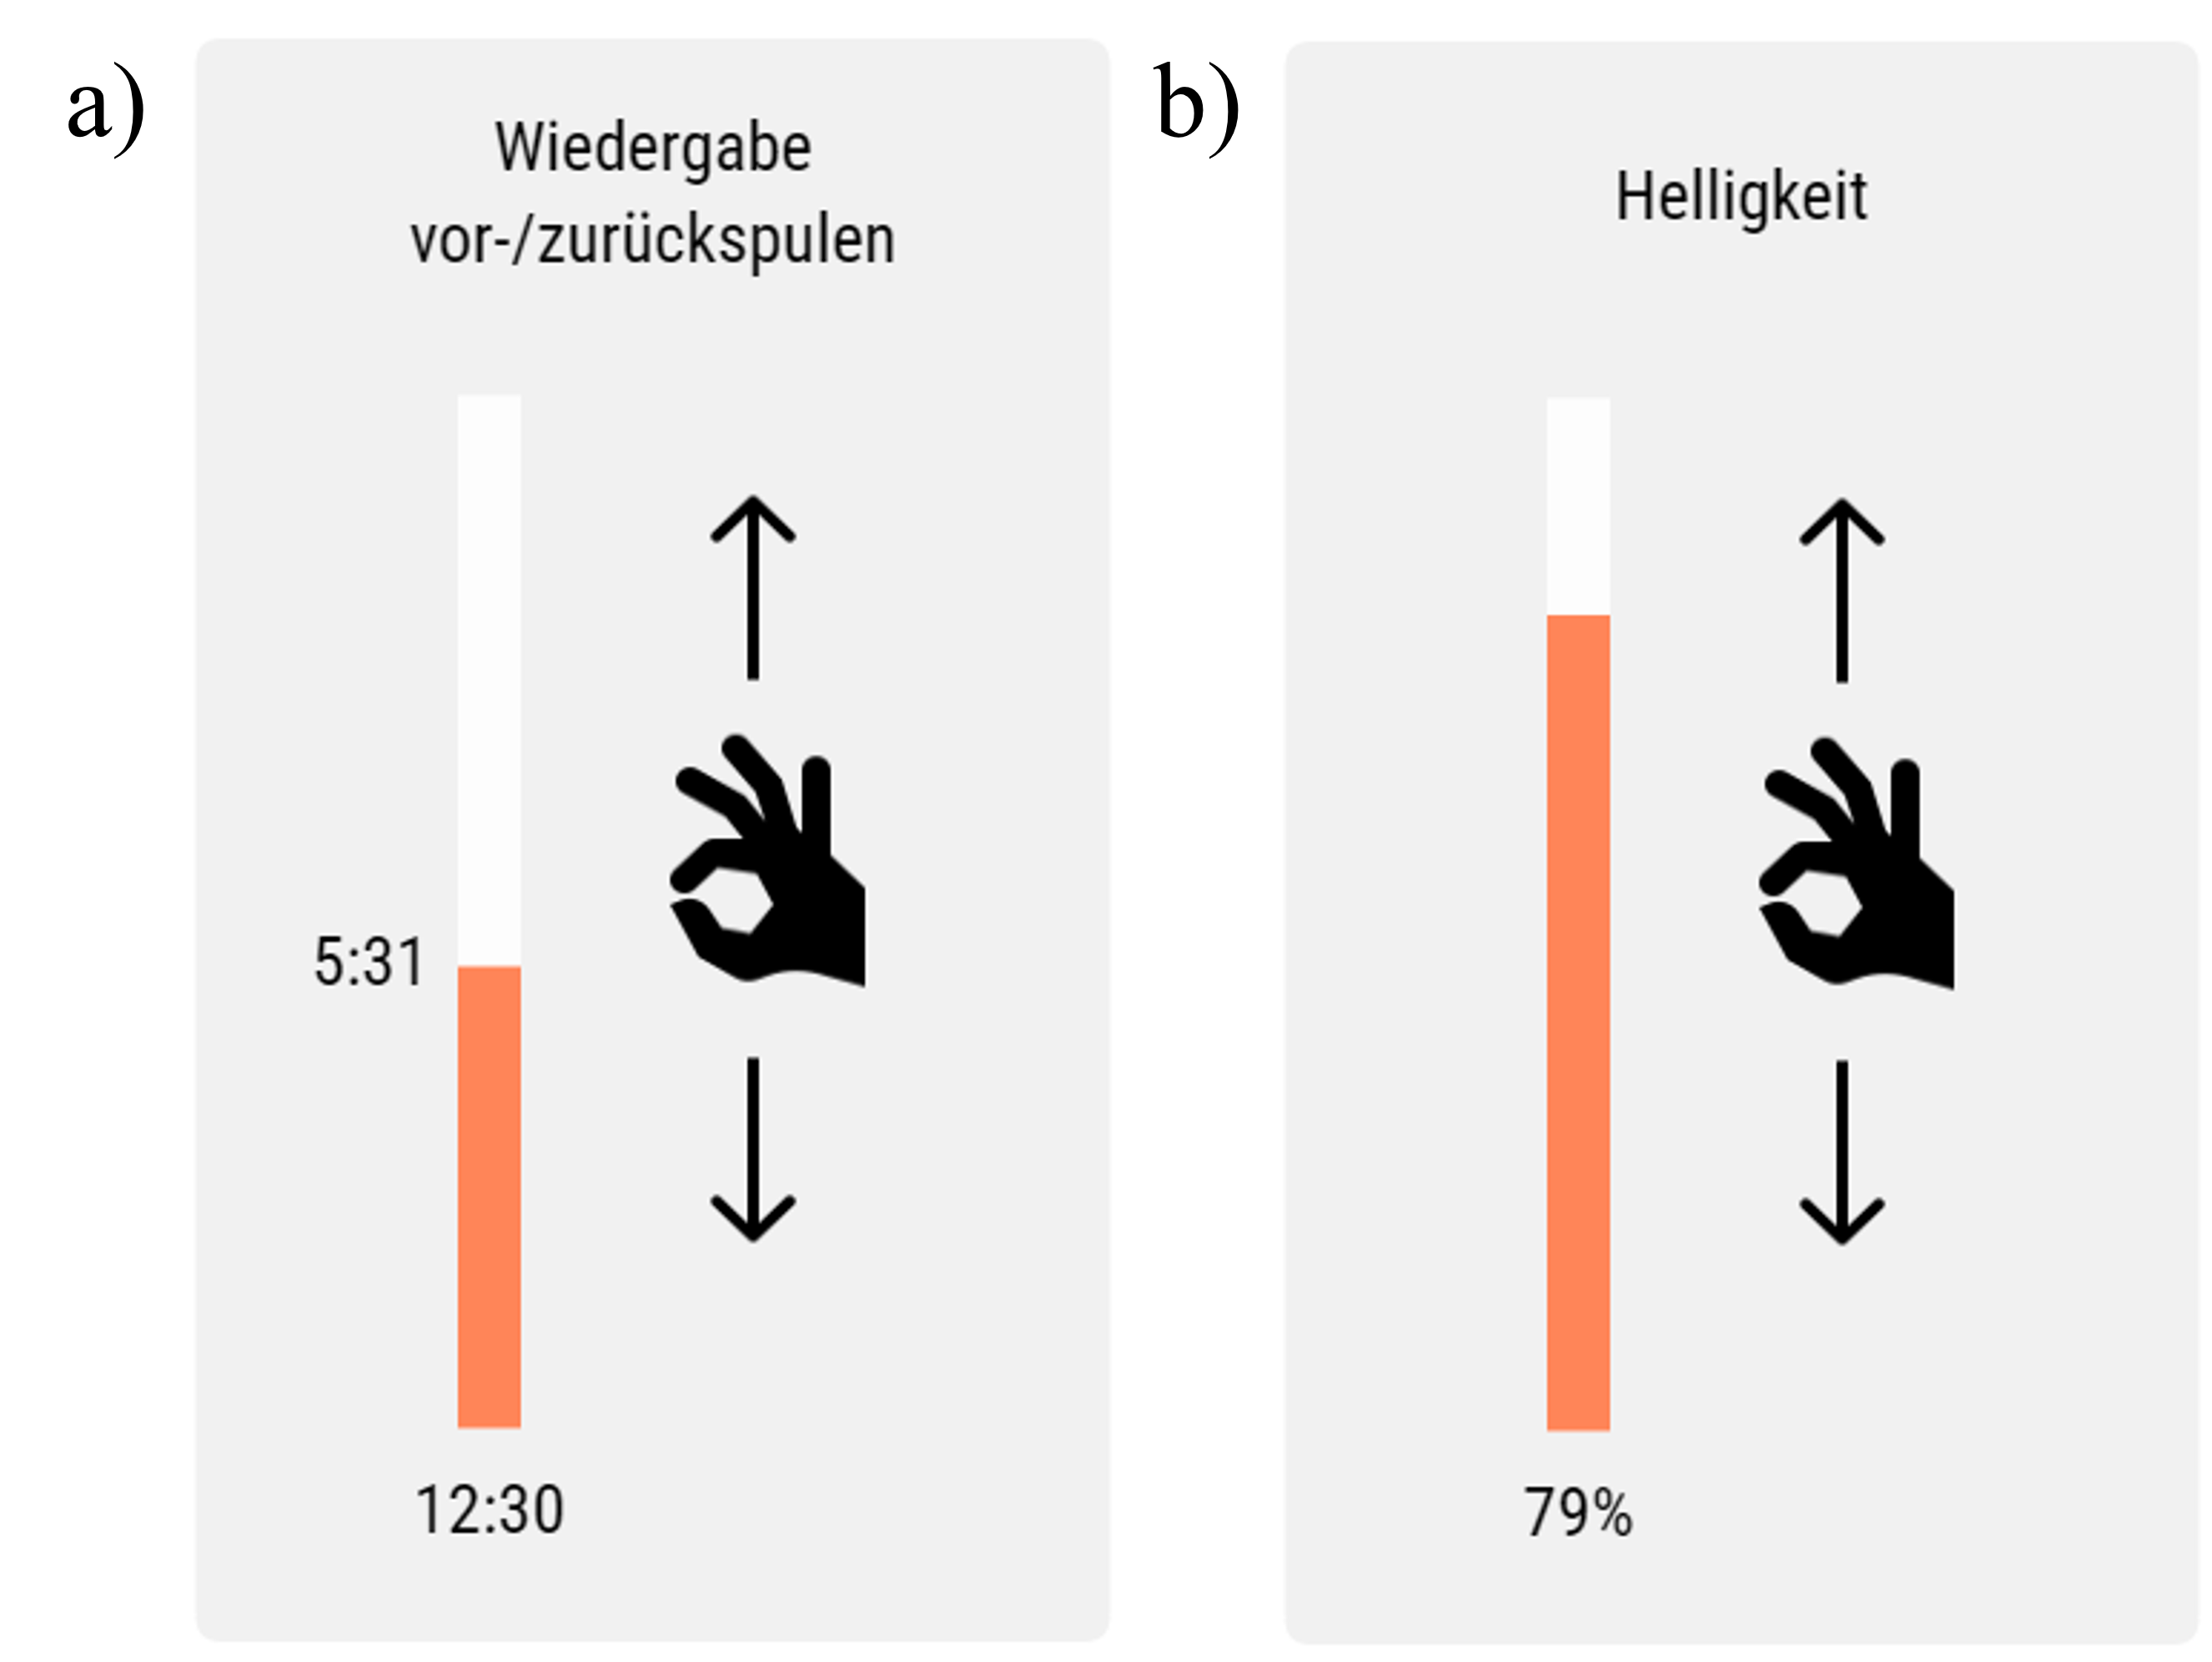
\includegraphics[width=0.5\linewidth]{content/diagrams/Slidertypen.png}
    \caption{Vergleich zweier Slider-Typen: a) zeigt einen zeitbasierten Slider zur Navigation innerhalb eines Videos, b) zeigt einen parameterbasierten Slider mit prozentualer Anzeige. Beide verwenden identische Interaktionsmechanismen bei unterschiedlicher semantischer Bedeutung.}    \label{fig:Slidertypen}
\end{figure}

Ergänzend dazu ist ein Button zur Steuerung der Wiedergabe implementiert, der als klickbares Menüelement realisiert ist. Dieser ermöglicht das Starten und Pausieren des Videos. Der aktuelle Systemzustand wird dabei durch eine visuelle Änderung des Icons kommuniziert, wie in Abbildung \ref{fig:Buttons} dargestellt. Der Button kann wiederholt aktiviert werden und verhält sich funktional analog zu einem klassischen physischen Bedienelement, ist jedoch in die Menüstruktur integriert.

\begin{figure}[H]
    \centering
    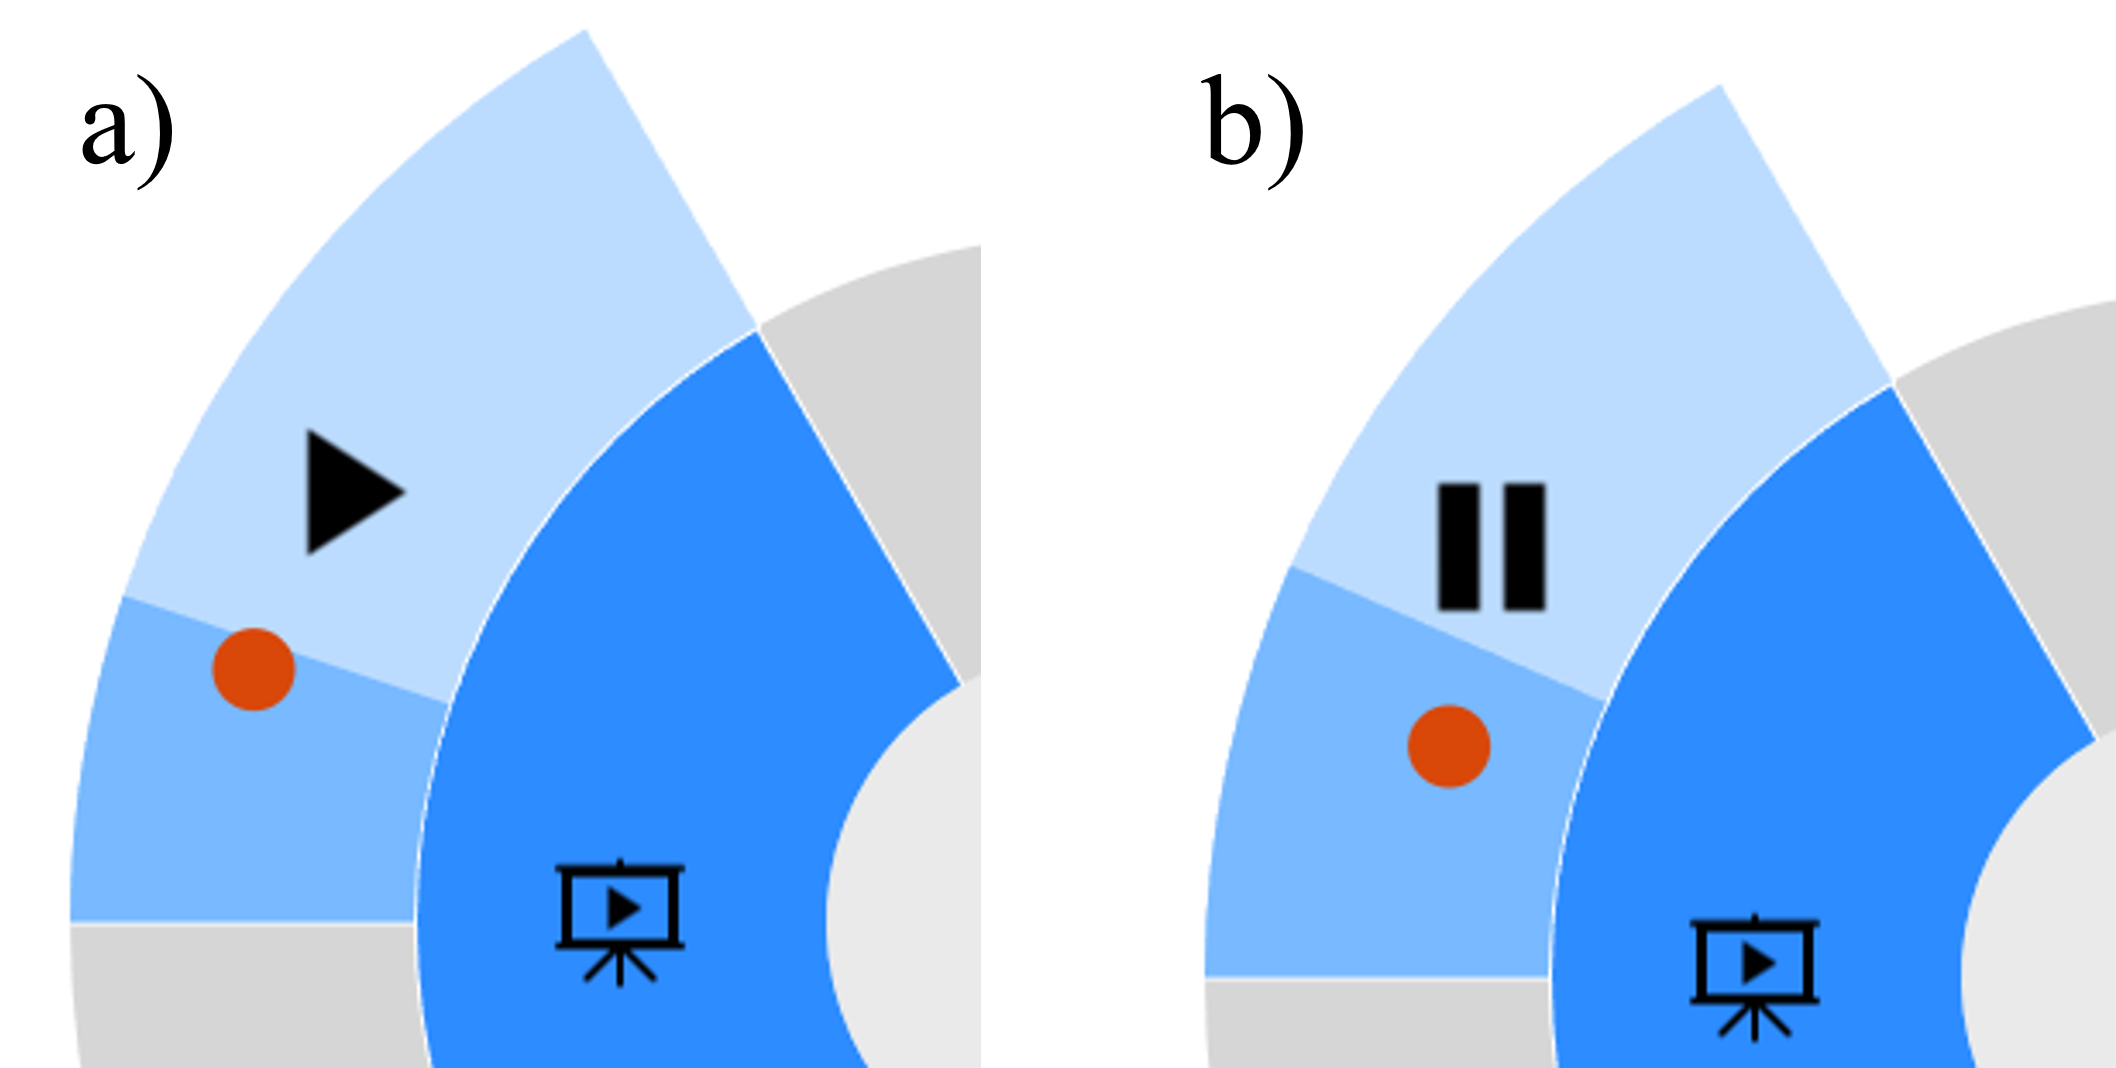
\includegraphics[width=0.5\linewidth]{content/diagrams/Buttons.png}
    \caption{Darstellung der beiden Buttonzustände. a) zeigt den Button, während das Video pausiert ist, b) zeigt den Button, während das Video läuft.}
    \label{fig:Buttons}
\end{figure}

{\color{red} Muss man für so einen Abschlusssatz ein Zusammenfassungsunterkapitel machen oder ist das ok, wenn das einfach bei Slider mit drin steht? }
% Überagang
Das beschriebene Interaktionskonzept kombiniert somit gestenbasierte Eingaben mit einer strukturierten Menüoberfläche. Durch die Kombination aus radialem Menü, hierarchischen Untermenüs und kontinuierlichen Steuerungselementen können unterschiedliche Interaktionsaufgaben innerhalb eines einheitlichen Systems abgebildet werden. Gleichzeitig bleibt die Interaktion vollständig controllerlos und in den räumlichen Kontext des MIR integriert.
